\subsection{Results and Analysis}

\begin{todolist}
\item mention a table that includes the number of qubits/layer/random parameter for each ansatz
\item describe more in figure \ref{Variance Local Cost}
\item analysis instead of describe
\item add the figures above (python notebook) for analysis
\item describe how alternating data leads to different result(s).
\end{todolist}

For the case of Local Cost Function and Shallow circuit, the variances of the ansatzes' gradient did not vanished when we attempt to increase the number of qubit.
In contrast, the ansatzes which don't have any restraint on the layer depth and cost function have the variances decay exponentially with the number of qubits.
In this case, the gradient of the cost function become flatter for each qubit in the ansatz.
Figure \ref{Variance Local Cost} shows the result of the experiment.

\begin{figure}
    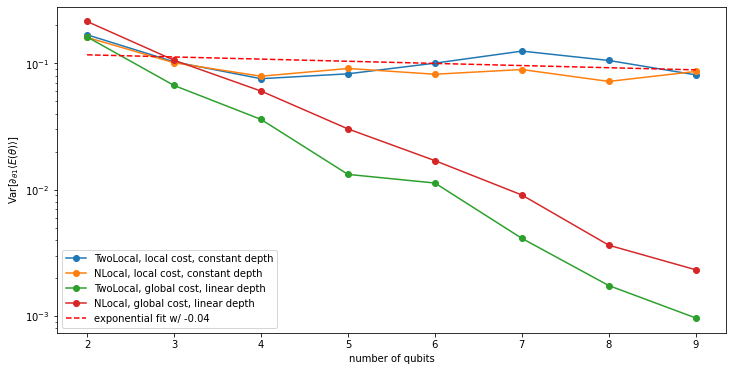
\includegraphics[width=\textwidth]{Artefact/Appendices/variancesLCF.png}
    \caption{
        Comparison of the variance values of the two ansatzes with and without Local Cost Function and constant depth.
        The ansatzes with Global Cost Function and increased depth have their gradient variances decay exponentially with the number of qubits. 
        In other word, the initial parameters has landed into a Barren Plateau.
    }
    \label{Variance Local Cost}
\end{figure}